\subsection{Auswertung EMG}
\subsubsection{Symmetrie-Index (SI): Bedeutung und Berechnung}

Der Symmetrie-Index (SI) ist eine Maßzahl, die den Grad der Asymmetrie zwischen zwei Körperseiten - beispielsweise der linken und rechten Seite eines Muskels - beschreibt. Er wird häufig in der Biomechanik, Physiotherapie und Sportwissenschaft verwendet, um muskuläre Dysbalancen zu bewerten.
Die Berechnung erfolgt mit folgender Formel:

\begin{equation}
    SI = \frac{|X_1 - X_2|}{\frac{X_1 + X_2}{2}} \cdot 100
\end{equation}
Wobei $X_1$ und $X_2$ die Mittelwerte der Muskelaktivität auf der linken ($X_1$) und rechten ($X_2$) Seite sind.
\\
Interpretation des Symmetrie-Index:
Ein höherer SI-Wert weist auf eine stärkere Asymmetrie zwischen den beiden Seiten hin.
Ein niedrigerer SI-Wert deutet auf eine gleichmäßigere Belastung und damit auf eine bessere Symmetrie hin.

\subsubsection{Symmetrie-Index vor und nach den Ausgleichsübungen}

Die durchschnittlichen Symmetrie-Index-Werte der drei analysierten Muskeln (Rectus femoris, Vastus lateralis, Vastus medialis) wurden vor und nach den Ausgleichsübungen berechnet. Zudem wurde ermittelt, wie viele Probanden eine Verbesserung des Symmetrie-Indexes (SI) zeigten:

\begin{table}[htbp]
    \centering
      \begin{tabular}{|p{8.455em}|p{5.135em}|p{5.135em}|c|}
      \hline
      \textbf{Muskel} & \textbf{Durchschnitt SI vor (\%)} & \textbf{Durchschnitt SI nach (\%)} & \multicolumn{1}{p{5.135em}|}{\textbf{Verbesserungen (Anzahl)}} \\
      \hline
      Rectus femoris & \multicolumn{1}{c|}{18.06} & 13.18 & 3 \\
      \hline
      Vastus lateralis & 24.24 & 18.70 & 3 \\
      \hline
      Vastus medialis & 17.84 & 15.05 & 3 \\
      \hline
      \end{tabular}%
      \caption{durchschnittliche SI-Werte}
    \label{tab:durchschnittliche-SI-Werte}%
  \end{table}%

\subsubsection{Interpretation der Ergebnisse}
\begin{itemize}
    \item Rectus femoris
    Der durchschnittliche Symmetrie-Index hat sich von 18.06 $\%$ auf 13.18 $\%$ verbessert.
    Bei allen drei Probanden wurde eine Verbesserung festgestellt.
    \textbf{"Interpretation:"} Die Ausgleichsübungen waren für diesen Muskel besonders effektiv, da die Symmetrie deutlich zugenommen hat.
    \item Vastus lateralis
    Der Symmetrie-Index hat sich von 24.24 $\%$ auf 18.70 $\%$ verbessert.
    Auch hier zeigten alle drei Probanden Verbesserungen.
    \textbf{"Interpretation:"} Der Vastus lateralis war vor den Übungen der asymmetrischste Muskel, aber die Übungen haben die Symmetrie erfolgreich gesteigert.
    \item Vastus medialis
    Der Symmetrie-Index hat sich von 17.84 $\%$ auf 15.05 $\%$ verbessert.
    Bei allen drei Probanden wurde eine Verbesserung festgestellt.
    \textbf{"Interpretation:"} Die Verbesserungen sind weniger ausgeprägt im Vergleich zu den anderen Muskeln, was darauf hinweist, dass der Muskel bereits eine bessere Ausgangssymmetrie hatte.
\end{itemize}

\subsubsection{Ergebnisse der EMG Messungen}
\begin{itemize}
    \item Die Ausgleichsübungen führten bei 3 von 4 Probanden zu einer Verbesserung der Symmetrie.
    \item Besonders der Rectus femoris und der Vastus lateralis profitierten von den Übungen, da bei ihnen die Asymmetrien am stärksten reduziert wurden.
    \item Der Vastus medialis hatte bereits vor den Übungen eine relativ gute Symmetrie, weshalb die Verbesserungen hier weniger ausgeprägt ausfielen.
\end{itemize}

\subsection{Mögliche Gründe für fehlende Verbesserungen des Symmetrie-Indexes}

Auch wenn bei diesem Datensatz durchgängig Verbesserungen festgestellt wurden, könnten in anderen Fällen folgende Faktoren dafür sorgen, dass keine Verbesserung des Symmetrie-Indexes erzielt wird:

\begin{itemize}
    \item 1. Unzureichende Wirksamkeit der Übungen:\\
    Die Übungen könnten nicht spezifisch genug gewesen sein, um die Asymmetrie in den betroffenen Muskeln auszugleichen.\\
    Eine ungleichmäßige Belastung während der Übungen könnte die Symmetrie sogar verschlechtern.\\
    %
    \item 2. Individuelle Unterschiede: \\
    Unterschiede im Fitnesslevel, in der Anatomie oder in der Bewegungskoordination der Probanden könnten den Effekt der Übungen verringern.\\
    Eine vorhandene Verletzung oder ein muskuläres Ungleichgewicht könnte die Symmetrie nicht vollständig ausgleichbar machen.\\
    %
    \item 3. Messfehler:\\
    Eine unpräzise Platzierung der EMG-Elektroden könnte zu falschen Werten führen, die den Effekt der Übungen verfälschen.\\
    Signalrauschen oder Störungen im EMG-System könnten die Datenqualität beeinträchtigen.\\
    %
    \item 4. Ermüdung oder Tageszeit-Effekte:\\
    Die Messungen vor und nach den Übungen könnten durch den Ermüdungszustand der Muskeln oder die Tageszeit beeinflusst worden sein.\\
    %
    \item 5. Lerneffekt:\\
    Die Verbesserungen könnten nicht auf die Übungen, sondern auf eine bessere Koordination der Probanden während der Messungen (Übungseffekt) zurückzuführen sein.
\end{itemize}


\subsection{Auswertung der Wägezelle}
\subsubsection{Quantisierung der Gewichtsverteilung}
% Kalibration der Wägezelle?
Die aus der Wägezelle übertragenen Gewichtsdaten der linken und rechten Seite sollen nun beschreiben wie sehr die linke oder rechte Seite beansprucht werden.
Da die EMG Messungen nicht gleichzeitig mit den Wägezellen Messungen durchgeführt wurden, können die Daten nicht direkt miteinander verglichen werden.
Um dennoch Erkenntnisse aus den Wägezellen Daten zu gewinnen, wurden folgende Überlegungen gemacht:
\begin{itemize}
  \item Die Phase in der sich die Person auf die Waage stellt und in der sie wieder absteigt wird für die Auswertung nicht berücksichtigt.
  \item Ein über die Zeit verteilt deutliche höheres Gewicht auf einer Seite entspricht einer stärkeren Belastung dieser Seite.
  \item ...
\end{itemize}

% \begin{align}
%   \int \Delta m(t) ~dt &\approx \sum_{i=1}^{n} \Delta m_i \cdot \Delta t_i
%   \label{eq:integral_differenz} \\
%   %
% \end{align}

\begin{figure}
  \centering
  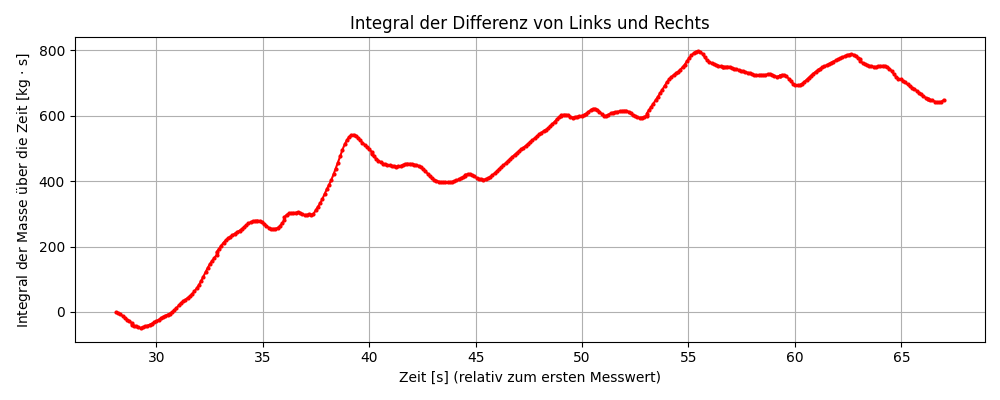
\includegraphics[width=0.8\linewidth]{img/pyplots/Integral der Differenz - Any.png}\\
  \caption{Integral der Differenz der Gewichtsverteilung von Any}
  \label{fig:weight_distribution_integral_any}
\end{figure}

In \autoref{fig:weight_distribution_integral_any} kann man eine deutliche Tendenz


